
\documentclass[12pt,a4paper]{article} % Use A4 paper with a 12pt font size - different paper sizes will require manual recalculation of page margins and border positions

% Generated with LaTeXDraw 2.0.8
% Mon Jun 17 19:00:40 EDT 2013
\usepackage[usenames,dvipsnames]{pstricks}
\usepackage{epsfig}
\usepackage{pst-grad} % For gradients
\usepackage{pst-plot} % For axes

\usepackage[left=1.3cm,right=4.6cm,top=1.8cm,bottom=4.0cm,marginparwidth=3.4cm]{geometry} % Adjust page margins
\usepackage{amsmath} % Required for equation customization
\usepackage{amssymb} % Required to include mathematical symbols
\usepackage{xcolor} % Required to specify colors by name
\usepackage{amsthm}
\usepackage{float}


\setlength{\parindent}{0cm} % Remove paragraph indentation
\newcommand{\tab}{\hspace*{2em}} % Defines a new command for some horizontal space


\title{Calculus Workshop - Limits Unit}
%----------------------------------------------------------------------------------------

\newtheorem{defn}{Definition}
\newtheorem{example}{Example}
\newtheorem{prop}{Proposition}
\newtheorem{exer}{Exercises}
\newtheorem{thm}{Therorem}
\begin{document}
\maketitle

\section{Limits} 
In order to prove things about limits, we need to have a precise, formal definition:
\begin{defn}
Let $f$ be a real-valued function of a real variable, $x$.  Let $a,L$ be fixed real numbers.  If for every $\epsilon >0$, there exists some $\delta>0$ such that
\begin{equation*}
|f(x) - L|<\epsilon 
\end{equation*}
whenever
\begin{equation*}
|x - a|<\delta 
\end{equation*}
we say that
\begin{equation*}
\lim_{x\rightarrow a} f(x) = L
\end{equation*}
\end{defn}
Now, let us parse this statement into English.  We are saying that given any specified tolerance ($\epsilon$), which can be arbitrarily small, we can find a distance $\delta$ so that if $x$ is within $\delta$ of $a$, then $f(x)$ will be within $\epsilon$ of $L$.  Loosely speaking, if $x$ is close enough to $a$, $f(x)$ will be close to $L$.  Pictorally:

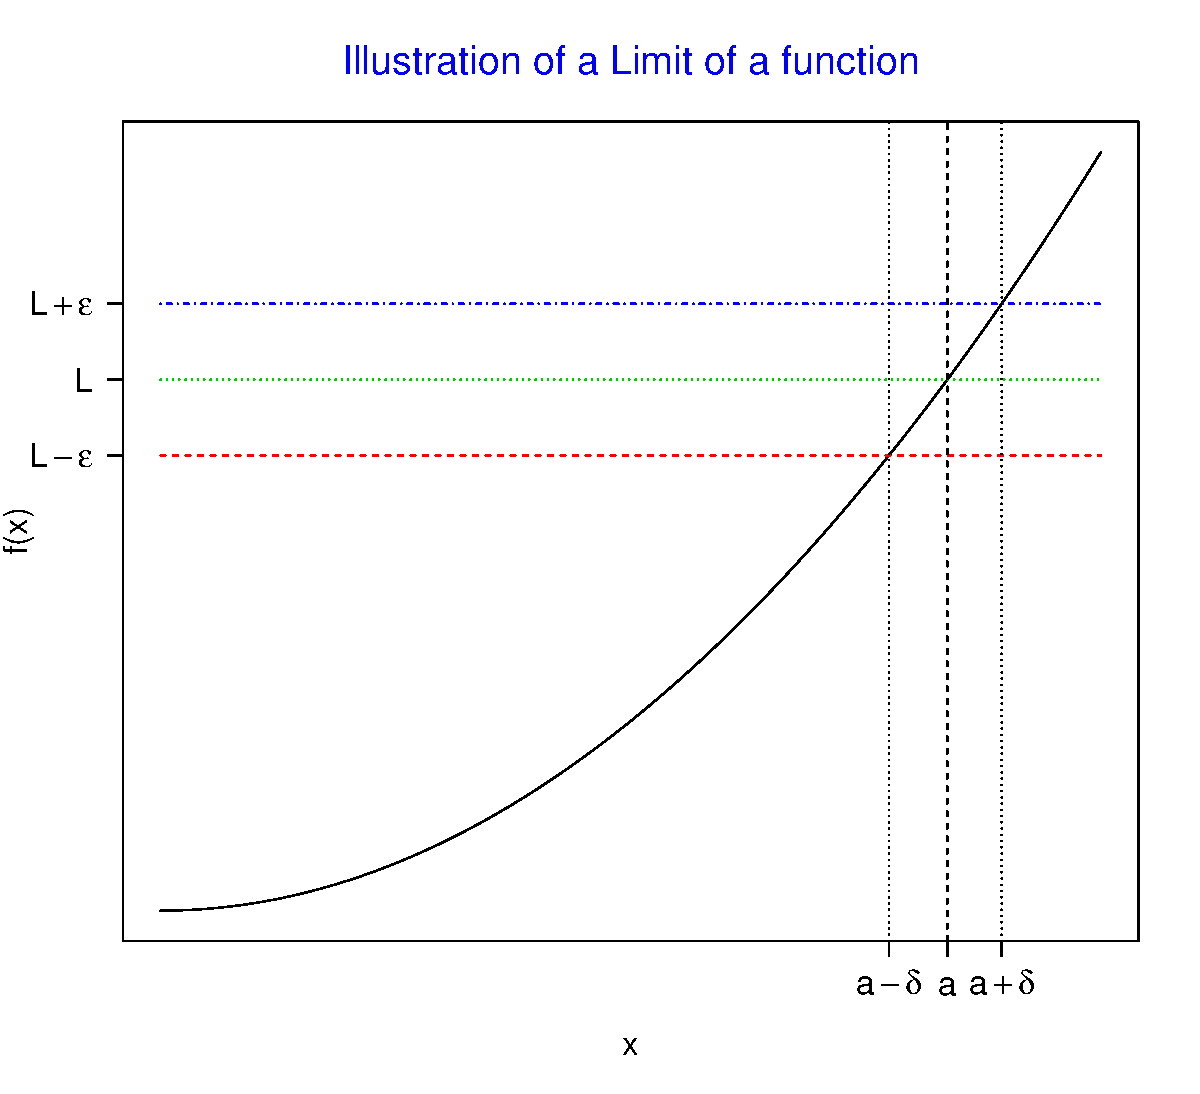
\includegraphics[height=3in]{limit.pdf}

The function pictured has a special property: it is \emph{continuous}.  We will give a formal definition of this in a moment, but it means that the limit of the function at a point is equal to the function value.  Let us look at another example, one that gives a little better idea of the utility of such a thing as a limit.  Consider\\

\begin{equation}
\lim_{x\rightarrow 0}\frac{\sin(x)}{x}
\end{equation}
This function is not defined at $x=0$, however, the above limit exists!  We can see this by looking at the graph of $\frac{\sin(x)}{x}$.  

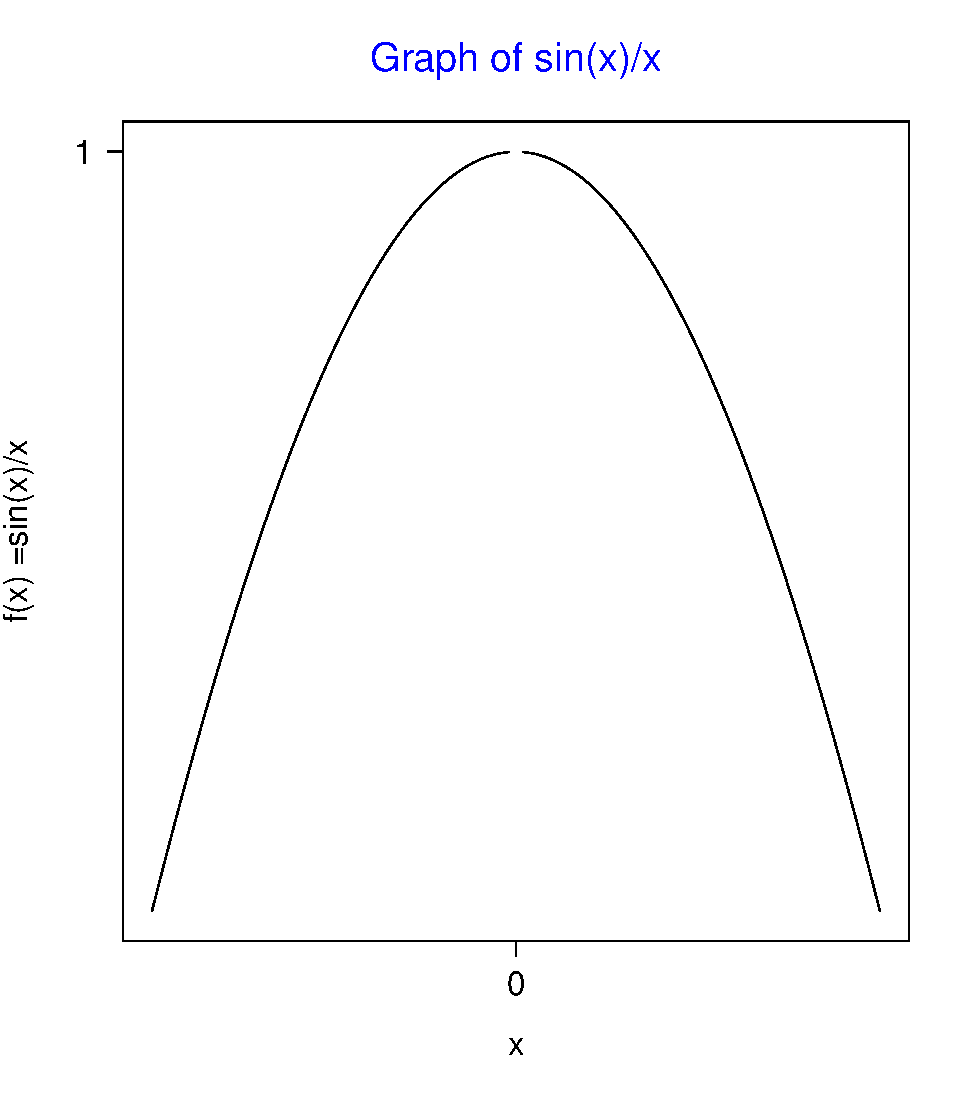
\includegraphics[height=3in]{sinxoverx.pdf}

The graph does not constitute a proof, but we can see that the graph approaches $1$ as $x\rightarrow 0$ from both the left and the right.    How \emph{do} we prove limits?


This brings us to our next topic:

\subsection{Proving Limits with $\epsilon$ and $\delta$}

In the previous section, we stated the formal definition of a limit.  When we wish to prove a limit, we may start with this definition.
\begin{example}
Prove that $$\lim_{x\rightarrow 3} 2x +4 =10$$.\\
\end{example}
The formal definition of a limit says that given any $\epsilon>0$, we must find $\delta>0$ such that $|2x+4 -10|<\epsilon$ whenever $|x-3|<\delta$.  When we prove a limit from the definition, we must always find an expression for $\delta$ in terms of $\epsilon$.  We begin with the inequality containing $\epsilon$ and 'work backwards':
\begin{eqnarray*}
|2x+4-10| &<& \epsilon \iff \\
|2x-6|&<& \epsilon \iff \\
2|(x-3)|&<&\epsilon \iff\\
|(x-3)|&<&\frac{\epsilon}2
\end{eqnarray*}
So we may set $\delta = \frac{\epsilon}{2}$.  Now we are ready for the proof:
\begin{prop}
$$\lim_{x\rightarrow 0} 2x + 4 =10$$
\end{prop}
\begin{proof}
Fix $\epsilon>0$ and set $\delta = \frac{\epsilon}{2}$.  Then if $|x-3|<\delta$:
\begin{eqnarray*}
|x-3|&<&\frac{\epsilon}{2}\iff\\
2|x-3|&<&\epsilon\iff\\
|2x -6|&<&\epsilon\iff\\
|2x +4 -10|&<&\epsilon
\end{eqnarray*}
\end{proof}

The 'working backwards' part is usually what is most confusing in the beginning.  It takes practice!  Here are some exercises:
\begin{exer}
Prove the following limits
\begin{enumerate}
\item $$\lim_{x\rightarrow 4} 7x+3=31$$
\item $$\lim_{x\rightarrow -3} x+5 =2$$
\item $$\lim_{x\rightarrow 1}{\frac{4}{5}x +\frac15=1}$$
\end{enumerate}
\end{exer}
Those examples were all \emph{linear} functions of $x$, and therefore have a certain simplicity.  Let's try another example:
\begin{example}
Prove $$\lim_{x\rightarrow 3} x^2 =9$$.
\end{example}
As before, we start with the definition and note that given $\epsilon>0$, we must find some $\delta>0$ so that $|x^2-9|<\epsilon$ whenever $|x-3|<\delta$.  We start with the $\epsilon$ term and work backwards:
\begin{eqnarray*}
|x^2-9|&<&\epsilon\iff\\
|(x+3)(x-3)|&<&\epsilon\iff\\
|(x+3)||(x-3)|&<&\epsilon\iff\\
\end{eqnarray*}
Now what?  In the previous examples, we could just 'solve' the inequality for the $|x-a|$ expression and get $\delta$ in terms of $\epsilon$.  We cannot do that here, because we would need $\delta=\frac{\epsilon}{|x+3|}$ and we cannot have $\delta$ in terms of $x$.  What we need to do here is to find a way to bound $|x+3|$.  The trick is that we are specifying $x$ 'close' to $3$ in choosing $\delta$.  We choose an arbitrary $\delta$, say $\delta=1$.  Now, if $|x-3|<1$:
\begin{equation*}
-1<x-3 <1 \iff
\end{equation*}
\begin{equation*}
 2<x   <4
\end{equation*}    
This means we can bound the $|x+3|$ term, when $|x-3|$ is less than $1$:
\begin{eqnarray*}
|x-3| &<& 1\Rightarrow\\
|x+3| &<& 7 
\end{eqnarray*}
Now, we are ready for the proof. We will set $\delta =\mathrm{min}\left(1,\frac{\epsilon}{7}\right)$, so that we know we have set $|x-3|$ to be \emph{at most} smaller than $1$, and our bound for $|x+3|$ above is valid:
\begin{prop}
$$\lim_{x\rightarrow 3}x^2 = 9$$
\end{prop} 
\begin{proof}
Let $\epsilon>0$ be fixed and set $\delta =\mathrm{min}\left(1,\frac{\epsilon}{7}\right)$.  (Note that this ensures that $|x-3|$ is both $<1$ \emph{and} $<\frac{\epsilon}{7}$ Then:
\begin{eqnarray*}
|x-3|&<&\delta\Rightarrow\\
|x-3|&<1& \Rightarrow\\
|x+3| &<& 7 
\end{eqnarray*}
So, we have that:
\begin{eqnarray*}
|x^2-9|&=&|x+3||x-3|\\
&<& 7|x-3|\\
&<& \epsilon
\end{eqnarray*}
\end{proof}
And now, it's your turn:
\begin{exer}
Prove the following limits:
\begin{enumerate}
\item $$\lim_{x\rightarrow 2} x^2-4=0$$
\item $$\lim_{x\rightarrow 2} x^2-3x+1=-1$$
\end{enumerate}
\end{exer}
\subsection{Limits at Infinity}
We now move on to defining limits at infinity.  We would like to understand the behavior of a function, say $f(x)$ as $x$ gets arbitrarily large.  Will $f(x)$ also increase indefinitely?  Will it decay to some constant value?  Or perhaps $f(x)$ will not achieve a limit at all.  How can we tell?  First we need a formal definition, so that we know \emph{exactly} what we mean when we talk about the limit of a function as $x\rightarrow\infty$:
\begin{defn}
Let $f:\mathbb{R}\rightarrow\mathbb{R}$. Let $L$ be a fixed real number.  If for every $\epsilon >0$, there exists some number $c>0$ such that
\begin{equation*}
|f(x) - L|<\epsilon 
\end{equation*}
whenever
\begin{equation*}
x>c 
\end{equation*}
we say that
\begin{equation*}
\lim_{x\rightarrow \infty} f(x) = L
\end{equation*}
\end{defn}
Now let's use this definition to prove a limit:
\begin{example}
Prove $$\lim_{x\rightarrow\infty} \frac{1}{x} = 0$$
\end{example}
Again, we work backwards.  Given some fixed $\epsilon>0$, we want to find some value $c$ so that if $x>c$, then $|\frac{1}{x}|<\epsilon$.  Without loss of generality, we can assume $x>0$ (we want to work with large values of $x$).  
\begin{eqnarray*}
\frac{1}{x}&<\epsilon \Rightarrow\\
x&>\frac{1}{\epsilon}
\end{eqnarray*}
so we simply set $c=\frac{1}{\epsilon}$.  Now we write the proof:
\begin{prop}
$$\lim_{x\rightarrow\infty} \frac{1}{x} = 0$$
\end{prop}
\begin{proof}
Let $\epsilon>0$ be fixed and set $c=max(0,\frac{1}{\epsilon})$.  Then:
\begin{eqnarray*}
x&>c\Rightarrow\\
x&>\frac{1}{\epsilon}\Rightarrow
\frac{1}{x}&<\epsilon
\end{eqnarray*}
\end{proof}
\begin{exer}
Prove the following limits:
\begin{enumerate}
\item $$\lim_{x\rightarrow\infty} \frac{8x+2}{4x+1} = 2$$
\item $$\lim_{x\rightarrow\infty} \frac{\cos(x)}{x} = 0$$
\item $$\lim_{x\rightarrow\infty} \frac{2x}{3x-1} = \frac23$$
\end{enumerate}
\end{exer}
\end{document}